\chapter{Information modeling}
\label{sect:uml}

In this Chapter we introduce some ideas and methods that have been designed
formally model the entities and relationships that are important for an
organisation. In particular, we will give a brief introduction into Unified
Modeling Language.

\section{Information models} 
An information model is an attempt to capture the essence of the real-life
thing or process in simpler, abstract terms. We have seen an example of an
information model in Chapter~\ref{sect:erd}, when we talked about
Entity-Relationship Diagrams, see also Figure~\ref{fig:erd}.
%
\begin{figure}[h]
\centering
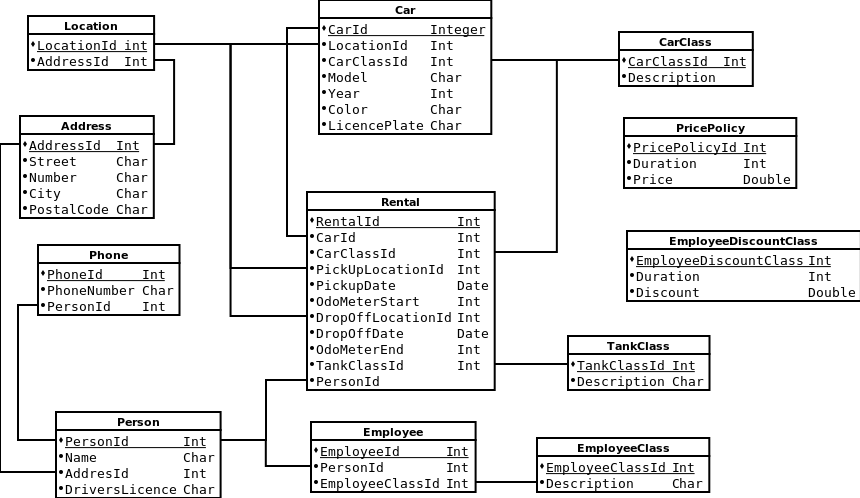
\includegraphics[width=\textwidth]{fig/schema.png}
\caption{An Enterprise-Relationship Diagram}
\label{fig:erd}
\end{figure}

Information models are often separated into three layers, that differ in their
level of detail and precision. The first type is \emph{conceptual}. Conceptual
models are often presented as text or schematic visualisations and their main
purpose is to communicate the bare essentials, for example to high-level
management. There is no formal language for conceptual models, although UML can
be used for this purpose. The second layer is the \emph{logical} information
model (LIM). A LIM describes all information elements in a structured way and
serves as a blueprint for development of for example, a database. A LIM is
typically platform-independent. That is to say, it does not depend on any
particular programming language, database system,  or other implementation
details. Again, UML can be used in this manner but the Entity-Relationship
Diagram of Figure~\ref{fig:erd} is also a good example. The last layer is the
\emph{physical} layer, which describes all technical choices including database
type and configuration input file format, connections to other databases and so
on. 




\section{Introduction to Unified Modeling Language}
UML is a formal graphical language that was developed in the 1990's to cope
with increasing complexity of large software projects. The idea is to
systematically capture all components and the typed relationships between them
in a formal graphical representation that would both be easy to create and easy
to understand. The idea was that ideally, a program can be defined in UML and
the software code can be generated automatically based on the UML
specification. The UML specification itself, is platform-independent and can be
transformed between for example database systems or operating systems.

Like information models in general, UML can be used in roughly three different
ways. It can be used as a sketch tool to outline the most important part of a
process or application. Sketches can be made on a whiteboard or a piece of
paper. Second, it can be used as a blueprinting tool that documents all
components of (for example) a database and the relations between it.  In this
case, it is common to use an UML drawing tool. The resulting document is then
part of the formal specification of a database (or other software system).
Finally, UML can be used as a programming language. Theoretically, if a system
is modeled in enough detail, the UML description can be translated to
executable code on any system where an UML translator  is available. In practice
this is cumbersome and not many applications are developed in that way.

Here we will focus on UML as a sketching tool and treat only a few of the most
important aspects of it. Nevertheless, these aspects can be useful to focus
one's thinking about complex systems or to communicate ideas and designs. Readers
interested in learning more about UML can refer to textbooks, such as that
by \citet{miles2006learning}. 

The main advantages of UML include its generality, understandability and wide
applicability. It can be used to model software, databases, but also the
structure of organisations or physical installations. A disadvantage is that
UML drawings quickly become too large and cluttered to interpret in full. A
more formal disadvantage is that UML is static, in the sense that there is no
algebra of manipulations that allow one to simplify or otherwise manipulate an
UML diagram automatically.

\subsection{Classes and Relations}
UML is used to describe \emph{classes} and their relations.  Term class is an
UML term, and would in the language we've developed in
Chapter~\ref{sect:relational} called an `entity type'. Information objects are
represented as blocks, and relations are represented as possibly decorated
lines between them. The relationships are decorated depending on their type.

The simplest type of relation is an \emph{association}. For example, the
following diagram displays an association between a pet and an owner.
$$

\includegraphics[height=7mm]{fig/pet_owner.png}
$$
Although the box labels are suggestive, in UML this diagram does actually
not say anything about who owns who, or any other property the association
might have. It merely states that a pet is associated with an owner.

\begin{terminology}{Association}
An association between two classes is a relation
that has no direction. It is represented as a solid line between
two information elements.
$$

\includegraphics[height=8mm]{fig/association}
$$
Associations are allowed to have an \emph{arity}, to be labeled, and to have a
direction (See Equation~\ref{eq:labeledassociation}).
\end{terminology}

Classes may be endowed with \emph{attributes} of a certain type. These
properties that may take different values for different elements of the class.
$$
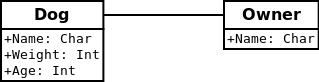
\includegraphics[height=15mm]{fig/pet_owner_attributes.png}
$$
So far, we have done nothing that we have not seen when we discussed
entity-relationship diagrams (Chapter~\ref{sect:erd}). This changes when
we add the \emph{arity} of an association. For example, we can annotate
the association between `Dog' and `Owner' to indicate that a single
Owner is associate with zero or more dogs.
$$
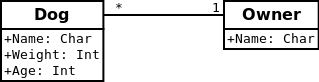
\includegraphics[height=15mm]{fig/pet_owner_arity.png}
$$
Here the asterisk stands for `zero or more' and the 1 stands for, well, one.
%
\begin{terminology}{Arity}
  The \emph{arity} describes the multiplicity on both ends of a relationship.  It
  expresses how many instances of one class can be associated with how many
  instances of another.  The arity is notated at the beginning and end of a
  relation. The notations used are as follows.
  \begin{itemize}
    \item $*$ means 0 or more
    \item $n$, with $n$ a number means `exactly $n$' (for example $n=1$)
    \item $n\ldots m$ means $n,n+1,\ldots,m$.
    \item $n\ldots *$ means $n$ or more.
  \end{itemize}
\end{terminology}

Relations can be labeled, in which case they possibly also gain a direction.
\begin{equation}
\vcenter{\hbox{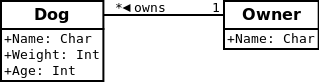
\includegraphics[height=15mm]{fig/pet_owner_labeled_association.png}}}
\label{eq:labeledassociation}
\end{equation}
Here, the owner `owns' a dog. The fact that it is the owner who owns is
signified by the arrow on the label.


Thus far we have discussed associations between classes. A second, more specific
type of relation is the \emph{composition} relation. This occurs when every entity
of a certain class is composed of elements of other classes. Composition is
graphically represented with a solid diamond on the side of the composed class.
$$
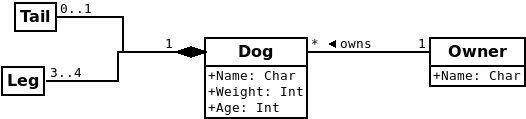
\includegraphics[height=25mm]{fig/pet_owner_composition.png}
$$
Here, a single `Dog' entity is contains 0 or 1 `Tail' entities and 3 to 4 `Leg`
entities. The fact that the lines coming from `Tail' and `Leg` combine before
entering the diamond has no significance; it is just a consequence of the
graphical representation.
\begin{terminology}{Composition}
Composition is an association that describes a part-whole relationship.
The line connecting the two classes is decorated with a solid diamond on the
side of the whole class.
$$

\includegraphics[height=8mm]{fig/composition.png}
$$
\end{terminology}

The last and slightly more complicated type of association we discuss here is
\emph{inheritance}. For any class with a nonempty set of attributes, we can
define a subclass by fixing one or more attributes. For example, we can define
the class `Animal'. If we fix the Boolean attribute `Mammal' to \yay{} and fix
the Species to Dog, we get an inherited class called `Dog'.
$$
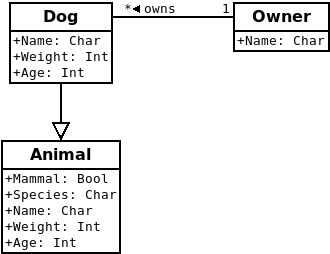
\includegraphics[height=45mm]{fig/pet_owner_inheritance.png}
$$
An equivalent way to think of inheritance is to say that any entity of class
`Dog' is also an `Animal' but not vice versa.

\begin{terminology}{Inheritance}
Inheritance is an association that defines a class-subclass relationship.
It is represented by an arrow, where the arrow points from the subclass to the
superclass.
$$

\includegraphics[height=8mm]{fig/inheritance}
$$
Here `A' is a subclass of `B'. An entity of class `A' has all attributes that
an entity of `B' has, but not the other way around.
\end{terminology}

\subsection{An application in Official Statistics}
\begin{figure}[t]
\centering
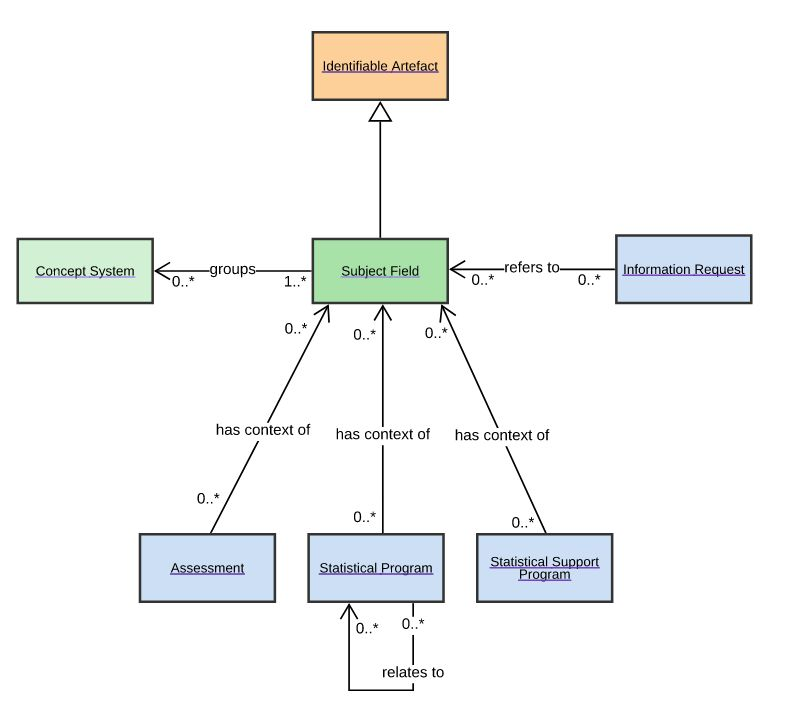
\includegraphics[width=0.7\textwidth]{fig/gsim.jpg}
\caption{The UML diagram surrounding `Subject Field' in the Concept Group of
the General Statistical Information Model. The open arrows indicate the
direction of the label in each association.}
\label{fig:gsim}
\end{figure}
The High-Level Group on Modernisation of Official Statistics (HLG-MOS) is an
initiative of the United Nations Economic Committee for Europe's (UNECE)
Statistical Commission. This initiative is an ongoing effort to both
standardize and modernize how official statistics are produced. HLG-MOS is
steered by a coaliltion of high level managers (typically director general or
deputy director general) who initiate several modernisation projects each year.

In one of these projects, called Generic Statistical Information Model
\hlink{https://statswiki.unece.org/display/gsim/}{(GSIM)}
an attempt was made to model all information objects in a statistical
organisation. The resulting UML diagrams can be found at
\begin{center}
\href{https://statswiki.unece.org/display/gsim/}{\code{https://statswiki.unece.org/display/gsim/}}.
\end{center}
The aim of this effort is not to create databases or software but to have a
reference document that describes the most important things and their
interrelations that are encountered by Official Statistical offices in a
standardized way.  You can think of it as a fancy glossary that can be reused
by statistical organizations. For example by using the same terms for the same
things in their documents and (international) communications. The idea is that
having a common understanding about all these concepts will facilitate common a
understanding of them; having a common understanding again, makes working
together in international context easier.


There are four main UML diagrams covering Business (design and planning of
statistical programs), Concepts (to define the meaning of what data are
measuring), Exchange (to catalogue information entering and exiting an
organization), and Structure (to structure information throughout the
statistical process). Figure~\ref{fig:gsim} shows a piece of the UML diagram
from the `Concepts' group, surrounding the term `Subject Field'. Each such diagram
als comes with a description of the main concept. For example, concept `Subject Field'
comes with the following description.
\begin{center}
\begin{tabular}{|p{0.45\textwidth}|p{0.45\textwidth}|}
\hline
\textbf{Definition} & \textbf{Explanatory text}\\
\hline
One or more \emph{Concept Systems} used for the grouping of \emph{Concepts and
Categories} for the production of statistics.
&
A \emph{Subject Field} is a field of special knowledge under which a set of
\emph{Concepts} and their \emph{Designations} is used. For example, labour
market, environmental expenditure, tourism, etc.\\
\hline
\end{tabular}
\end{center}


%%%%%%%%%%%%%%%%%%%%%%%%%%%%%%%%%%%%%%%%%%%%%%%%%%%%%%%%%%%%%%%%%%%%%%%%%%%%%%%
\section*{Where are we?}
The term `information modeling' refers to a set of techniques that allow one to
systematically describe complex systems. This can be done in ways that vary
from sketchy and high-level to formal and detailed approaches.  The Unified
Modeling Language supports all these approaches and lets the user decide what
level of detail is sufficient for their purpose.

\section{Exercises}
\label{sect:exinfomodel}

\begin{enumerate}
\item Describe the classes and relationships between them for each of the
following UML diagrams.
\begin{enumerate}
\item
$$
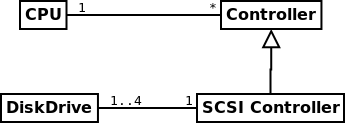
\includegraphics[height=25mm]{fig/ex_2_computer.png}
$$
\item
$$
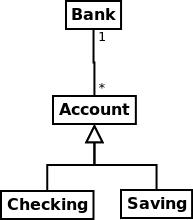
\includegraphics[height=45mm]{fig/ex_3_bank.png}
$$
\end{enumerate}
\item Complete the UML diagram of Figure~\ref{fig:erd}, see also Case~\ref{sect:schema} for a
full description. You can draw your own diagram or use the diagram on page~\pageref{pg:diagram}.
\end{enumerate}
\hfill{}Check your answers on page~\pageref{sect:ansinfomodel}.

\newpage
\begin{figure}[!h]
\centering
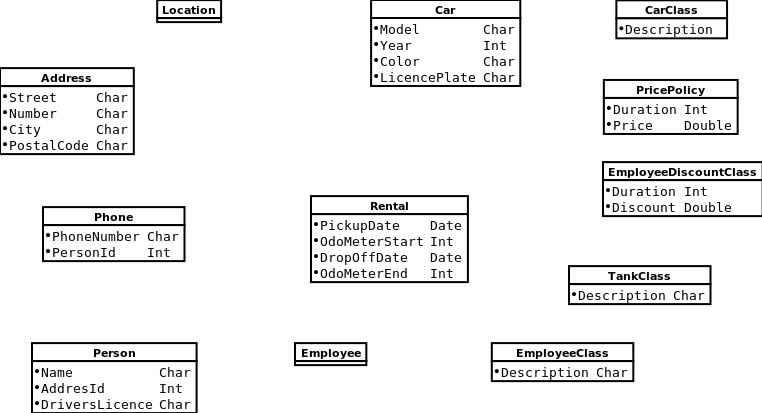
\includegraphics[height=0.8\textwidth,angle=90]{fig/uml_exercise.png}
\end{figure}
\label{pg:diagram}




